\begin{figure}[t]
  \begin{subfigure}[b]{0.45\textwidth}
    \centering
    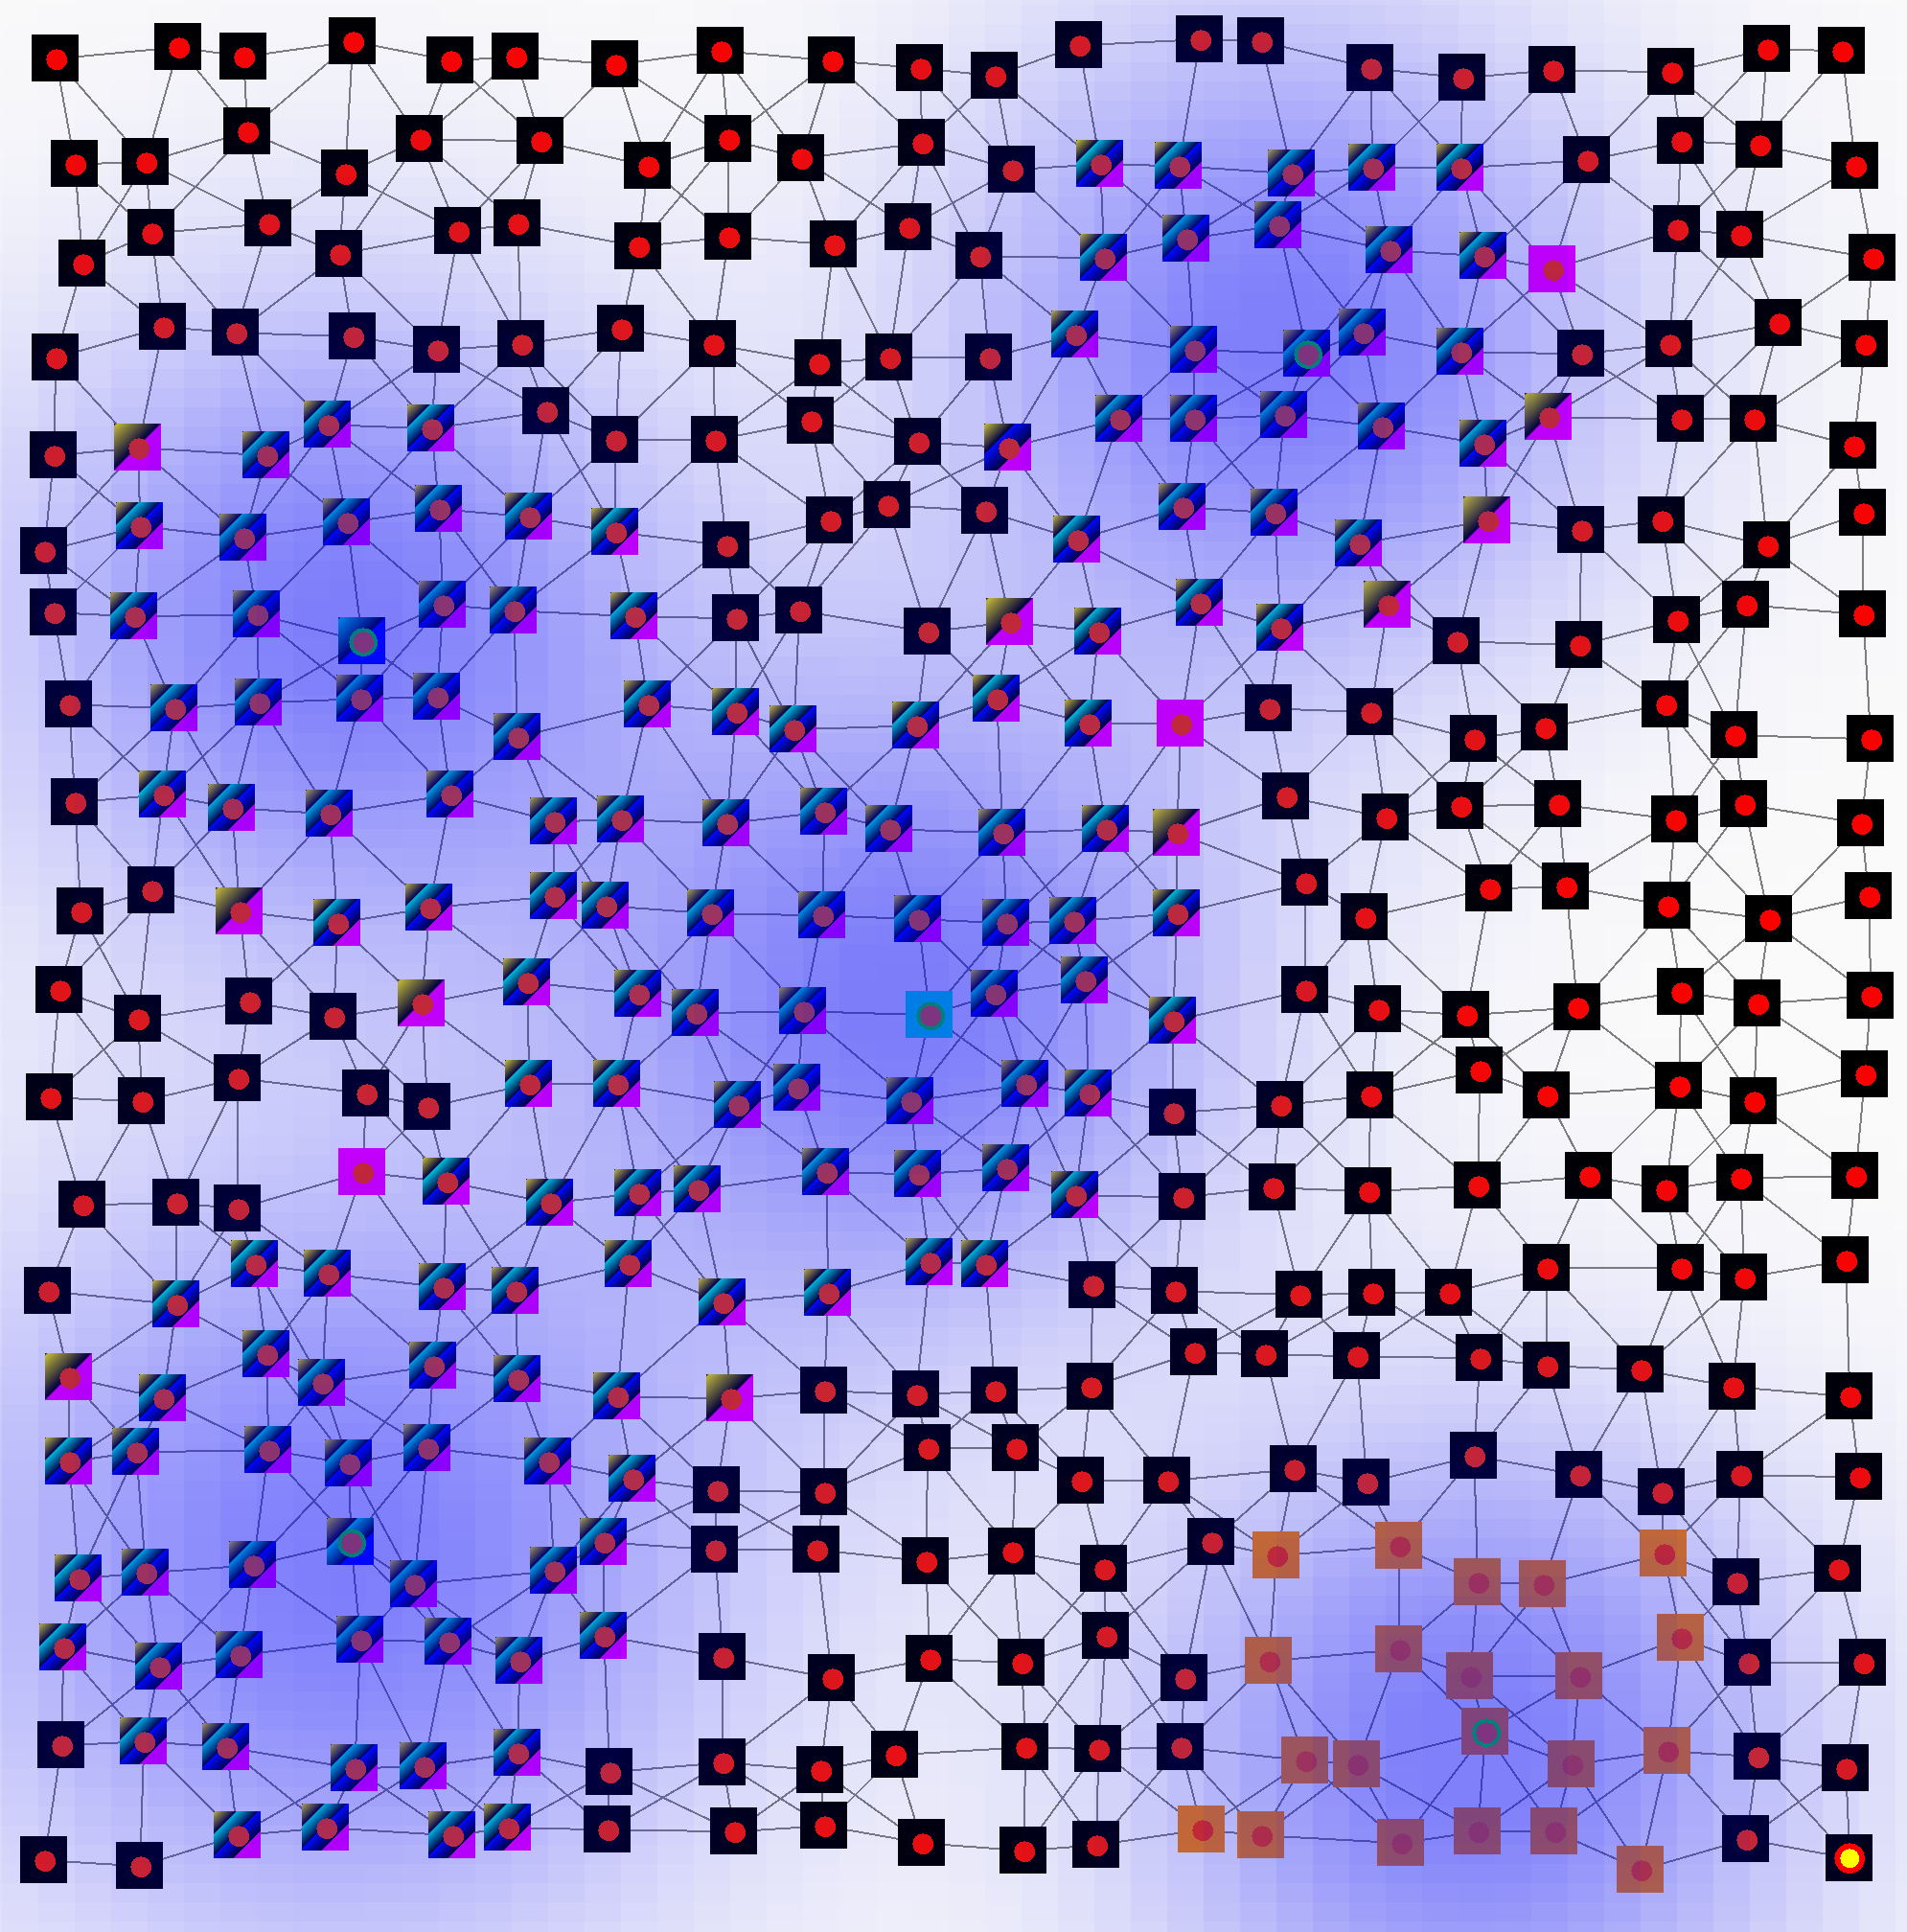
\includegraphics[width=\textwidth]{papers/swarm-intelligence2021/img/simulation-execution.png}
  \end{subfigure}
  \begin{subfigure}[b]{0.45\textwidth}
    \centering
    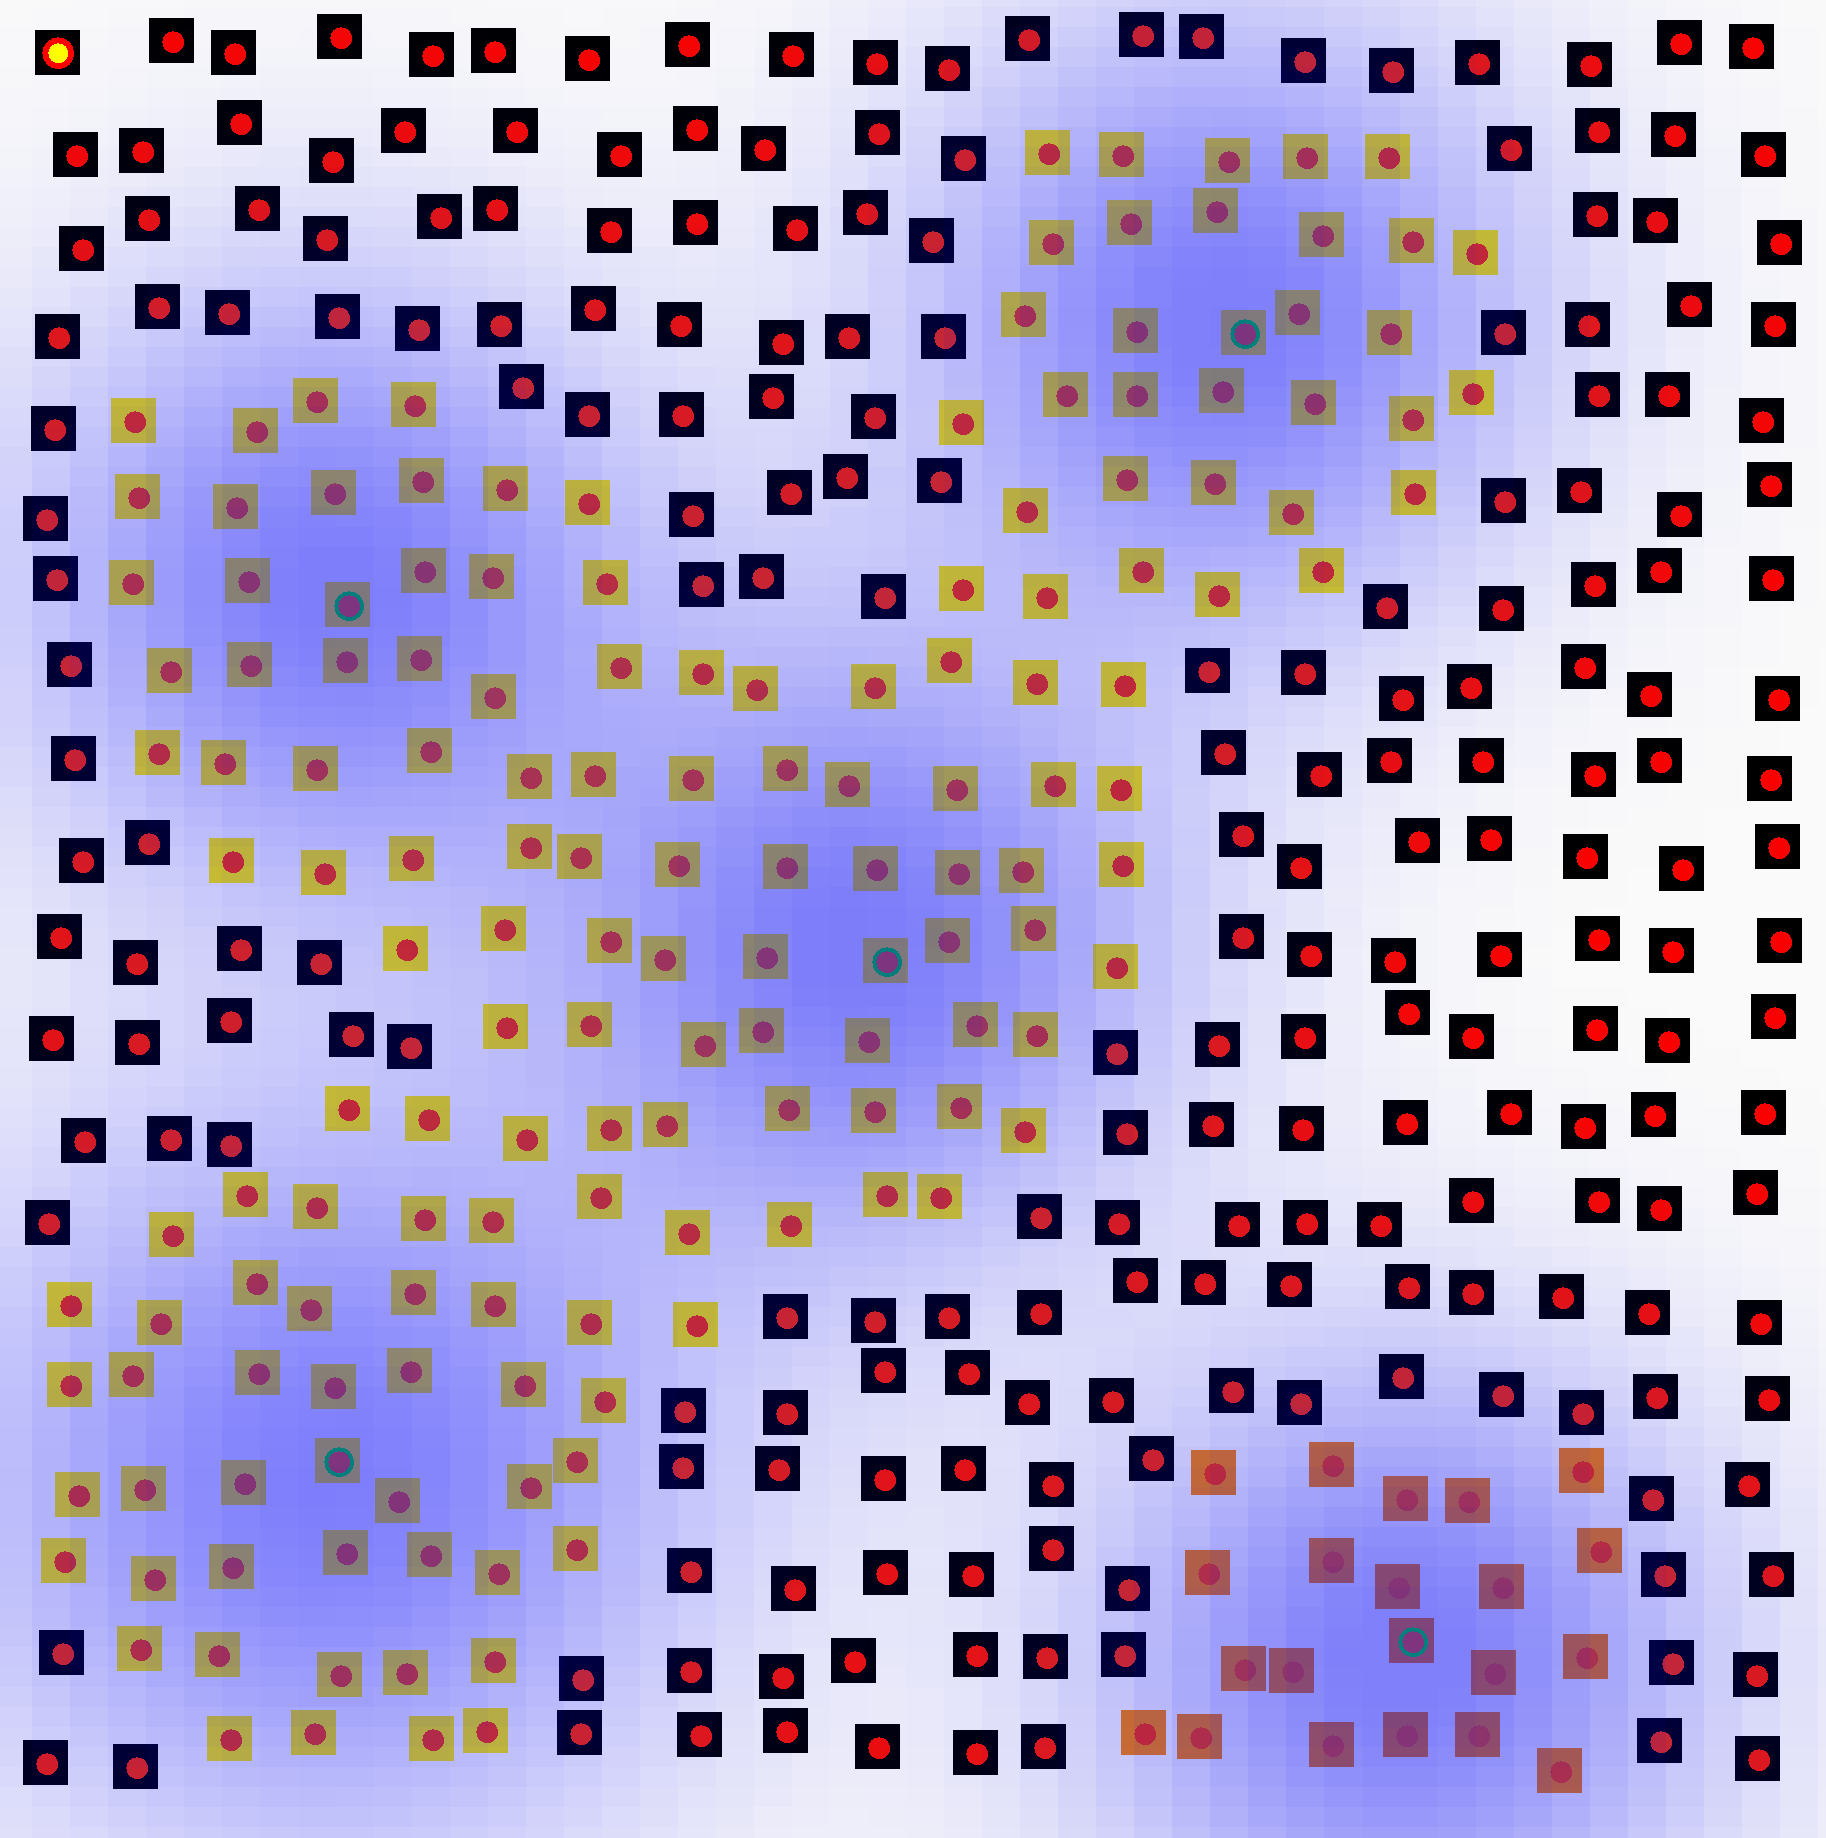
\includegraphics[width=\textwidth]{papers/swarm-intelligence2021/img/after-merge.png}
  \end{subfigure}
  \centering
  \caption{Snapshots of simulation executions. 
  The colour of the square identifies the cluster id found in that point. 
  Black colour means no cluster. 
  The green circle means that the node is a candidate. 
  The blue gradient circles are a graphical representation of temperature distribution. 
  On the left is shown a snapshot of a simulation before the merge policy has been applied (multiple clusters per point are found). 
  On the right, there is the snapshot of the same simulation after the merge policy action.}
  \label{fig:simulation-snapshot}
\end{figure}